\documentclass[../physical_computing.tex]{subfiles}

\begin{document}

\chapter{Starting point}

\section{What is Physical Computing?}
\label{sec:what_is_physical_computing}

Science and Engineering all about making connections between nature and mathematics. A successful scientific theory makes a connection between the behaviour of some real world hardware in an experiment and the properties of an abstract mathematical system that reproduces what is seen in that experiment. The starting point is observations about the real world hardware, and the end point is a mathematical model exhibiting the same behaviour, and perhaps predictive power. In engineering it is the same process in reverse. You start with an abstract idea that you want a real world system to replicate, and your end point is the realisation of that real world system - a machine. So science and engineering are both about relationships between nature and mathematics. In order to do either effectively, it is sometimes best to start from the simplest building blocks. Conceptually, the simplest abstract system is one that can only be in two states, say true or false. A two state system like this is called a bit. Bits turn out to be the basic currrency of computers that are some of the most sophisticated machines that engineers have produced, and have started the information revolution. In this book, we will be mostly concerned at first with bits and how to represent them using electronic circuits. We will catch glimpses of what those electronic circuits can do for science, and how they can be used as tools for building better abstract models of reality, also known as scientific theories.

The manipulation of these representations of bits using circuits is called digital signal processing (DSP). In classical digital signal processing, ranges of voltages on wires are used to represent the values of bits. For example, in 3.3V CMOS logic, the convention is that any voltage between $\rm 2.0\,V$ and $\rm 3.3\,V$ represents logic $1$, or true, any voltage between $\rm 0.0\,V$ and $\rm 0.8\,V$ represents logic $0$, or false. Just as the bits themselves are represented by classical voltage ranges, the operations on the bits are represented by circuits. For example, the simplest abstract digital operation I can think if is NOT, where if the input is a $0$ then the output is a $1$ and vice versa. An implementation of a NOT in a digital circuit must generate an output between $\rm 0.0\,V$ and $\rm 0.8\,V$ from an input between $\rm 2.0\,V$ and $\rm 3.3\,V$, and vice versa. Though of course digital circuits have become incredibly sophisticated, we shall show that all of them are made up of three basic circuit elements - gates, registers and oscillators. So the fundamental building blocks of classical computers are fewer in number than the fundamental building blocks of the Universe in particle physics!

In the first part of this book, we will learn to design and build digital circuits out of these three basic building blocks. The tasks that can be carried out by these circuits will be very simple, but I hope that by understanding the basic principles of how these blocks are combined, you will be able to see how these ideas can be generalised to far more complex systems. Forty years ago you would have needed a soldering iron, breadboard, or wire wrapping tool to assemble your circuits. We will instead use a more modern approach, and that is to make use of a hardware description language (HDL). This language enables us to describe the properties of the system we would like to represent. We then use computer software that translates our hardware description language code into a file called a bitstream that is used to configure a flexible device called a field programmable gate array (FPGA). Once programmed, the FPGA implements the digital circuit that represents the abstract system we described with our HDL code. This FPGA chip can be obtained housed on a development board with a variety of inputs and outputs that allow us to verify that the digital circuit is faithfully representing the operation of the digital circuit we described in our HDL code. You will also learn how exist half way between the abstract system and its hardware representation by simulating the behaviour of the digital circuit before you actually program the hardware device. In industry, hardware description languages are also used to design more specialised chips such as application specific integrated circuits (ASICs) and even entire processor cores. So, learning how to program FPGAs with hardware description languages (HDLs) is a useful and transferable skill. 

In the second part of this book, we will learn how to make use of HDL code that others already wrote to describe sophisticated circuits combined with HDL code that we wrote ourselves. An analogy is in computer programming, where you rarely write every line of the code you are using yourself; instead you make use of libraries and routines that were written by others. In particular, we will implement a soft core processor called MICROBLAZE on our FPGA, and we will learn how to interface our own HDL code to the microblaze core. MICROBLAZE is a fully functional processor core, so in order to operate correctly it will need programming. We will learn to program our microblaze core in C, a high level computer language that is particularly suitable to working directly with digital hardware. We will learn the C programming that is needed for this task as we go along.

In the last part of the book, we consider an important generalisation of digital signal processing, called quantum computing. I said at the beginning that the basic currency of DSP is the bit, that can take two different values. What happens if we try and represent a quantum system using classical bits? For example, we might have a system consisting of an electron for which the z component of the spin can be either up or down, so that the states are $\Ket{\uparrow}$ and $\Ket{\downarrow}$. However, notice that in quantum mechanics $\left(\Ket{\uparrow}+\Ket{\downarrow}\right)/\sqrt{2}$ is also a possible state of this system. Therefore, classical bits are not suitable for representing the state of a quantum spin. This example leads us to the more general abstract concept of a qubit, a system that can be in any linear superposition of two orthogonal states. It turns out that qubits can be manipulated using quantum circuits to perform computing tasks that are impossible with classical digital signal processing. We shall in the last part of this course learn more about the building blocks of quantum computers, and some of the problems encountered in trying to realise them in practice.

In summary, this book is part practical and part theoretical. The practical aim is to teach you the fundamentals of hardware description languages and computer architecture. These are skills you can use later for very practical purposes, like getting a job. The theoretical part is acquiring some useful knowledge that is a little off the beaten track, particularly for pure scientists, and understanding where we might be going next. The world of digital signal processing is colliding as we speak with the world of quantum mechanics, so this is an exciting time to be alive.

\section{What is this course?}
\label{sec:whatisit}

A course at University is intended to take the student on a journey between some starting point, a body of knowledge and skills which it is presumed they already have, to some finish point, where the student has learned some new material with some intended purpose. Many courses make the mistake of assuming the starting point is no knowledge at all! This is the safest bet for an academic, but it has two immense disadvantages. First, ignoring the student's existing knowledge means you end up re-teaching material, costing you precious time. Second, the student's existing knowledge may be in some context that they have never questioned. Pointing out that there is a wider world out there that they have not explored may pique their interest and motivate them to devote energy and time to working in your course. An under-appreciated reality of teaching is that it is in part the art of seduction. Students will not work for you unless you can succeed in motivating them to do so.

This course will attempt to raise your enthusiasm level by pointing out that what you probably know about computing is almost certainly confined to an artificial and some would say Utopian environment. Learning how to do computing outside this environment, in the real `physical' world is liberating and fun. Furthermore, many of the applications of computers, or more generally of digital circuits and algorithms, underpin some of the worlds most interesting machines and experiments, from spacecraft to gravitational wave detectors. We will in this course explain the senses in which these statements are true, and we will learn some basic techniques in what I call `physical computing'.

\section{Analysis of a simple program}
\label{sec:projectforstudents}

Most of you will have done a course in computer programming using a high-level language such as PYTHON. Below is a code listing that I lifted from an online programming course for undergraduates.

\begin{minted}{python}
import numpy as np
from matplotlib import pyplot as plt

ys = 200 + np.random.randn(100)
x = [x for x in range(len(ys))]

plt.plot(x, ys, '-')
plt.fill_between(x, ys, 195, where=(ys > 195), \
facecolor='g', alpha=0.6)

plt.title("Sample Visualization")
plt.show()
\end{minted}
The program produces this graphical output.
\begin{figure}[h!]
    \centering
    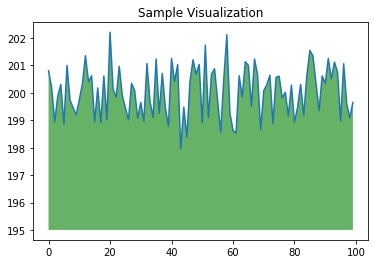
\includegraphics[width=0.8\textwidth]{chapter_1/figures/pythongraph.jpg}
    \caption{Graphical output of the PYTHON program}
    \label{fig:pythongraph}
\end{figure}

Let us analyse this program. First, its job is to make a plot of some random numbers. It probably isn't important exactly how long the code takes to produce this plot, as long as it isn't so long that it could have been done more efficiently without the computer. It also probably isn't critical that the program takes the same amount of time to produce this output every time it is run. 

The program makes use of some imported packages \texttt{numpy} and \texttt{matplotlib}, for mathematical functions and graphical output respectively.
It is somebody else's problem to implement these library functions. The \texttt{matplotlib} plotting function will only work if the computer has a way of outputting graphics. When I ran this code, the graphics appeared in my web browser, but this was because I was using Jupyter notebook; other python environments would have put the graphics in a separate window. 

Other observations about the program might seem obvious, but perhaps only because you have always taken them for granted. First, the program executes by default from top to bottom. Occasionally, there is a command that causes the code to go into a loop, so for example when the values of \texttt{ys} are generated, the
command \texttt{randn} generates 100 random numbers, so this random number 
generator loops around and runs 100 times before the program moves to the next
line of code. Similarly for the next line, which generates 100 values of \texttt{x}. All high-level programming languages feature loops, which cause code to execute multiple times. Another high-level programming concept is a conditional, meaning code that executes under some condition, but not if that condition is not satisifed. Loops and conditionals are so ubiquitous that you take it for granted that programs will utilise them. For that matter, you also take it for granted that code will execute from top to bottom.

Other things you might take for granted are particular to PYTHON. Notice how variables such as \texttt{x}, \texttt{ys} and \texttt{facecolor} represent data of different types, and that the type of data they represent is set automatically by PYTHON when the variables are defined. You don't generally have to declare what type of data a particular variable is going to be set to before that variable is used, PYTHON figures things out on the fly. In this respect, PYTHON differs from other high level languages like C or C++; in those languages you need to DECLARE a variable, including its data type, before you use it. You might think about whether this characteristic of figuring out variable types when they are first used is always a good thing, or whether perhaps it might occasionally cause problems.

The structure of high level computer languages generally comes about from them being intended for programming computers of a particular type. For example, most computers revolve around a very small number of processor cores which do all the calculations. Of course on a modern computer this may be less true than it used to be; there are often many cores on a CPU, and that doesn't include the GPU chip, where there are hundreds or thousands of cores that are more special purpose. In general, however, the architecture we imagine in a computer is that of a processor doing all the calculations, and input data and commands being piped in to this processor in sequence, and output form the processor coming out, so to speak, of the other side.

However, things do not have to be this way. In a more general calculating circuit, you can imagine the input data feeding in to the circuit through multiple parallel paths into a variety of different elements that all do things to subsets of the data at once. Such a circuit could be vastly more efficient than the gridlock that occurs when everything has to be stuffed in to a small number of processor cores. However, there is a price to pay, which is that the calculations in all these elements must be coordinated with each other, so that the outputs of the elements may combined and fed into yet more elements so that more calculations can be done, but on the right numbers. This way of doing things is potentially far more powerful than a conventional single processing unit architecture, but the programming of such a machine is vastly more complex as well. And, consider, the arrangement of the calculating elements for a particular computation may also need to be optimised for the efficiency of that computation. For the next computation, you may want to arrange the circuit differently.

So, in this course, we will consider the construction of digital circuits that do calculations. These circuits are literally wires connecting very fundamental building blocks. Until the 1980s. digital circuits were assembled using literal physical wires or circuit boards, connecting these fundamental blocks together. If you wanted a new circuit, you had to build it out of hardware. In the 1980s, however, large scale integration of digitial hardware led to a more abstract way of doing things. You described the digital circuit that you wanted using a new type of language, a Hardware Description Language (HDL). By a wierd stroke of luck I programmed early circuits of this type, which were called PALs, or programmable arrays of logic, using an early HDL called ABEL, when I was doing work experience at school. I had no idea that I would wind up using it's direct descendent, called VHDL, a far more advanced hardware description language, in my physics research more than 35 years later. Life is strange sometimes. Anyway, the hardware description language literally permits you to build a digital machine. You are building hardware, using a language.

Having built the hardware, in simple cases, you just pipe the data in, and the desired output appears at the other end of your digital machine. This has two great advantages. First, it is extremely fast. There is no operating system or other environment to slow down the process. Second, often the calculation takes exactly the same amount of time every time it is executed. This makes this type of machine suitable for use in situations where the output of the calculation is used to control the state of something critical, like a physics experiment, where unexpected delays cause glitches which may cause the machine or experiment to stop working.

In more complex cases, your machine may grow to resemble a computer, and you may need to write more code, this time perhaps in a high level language, to program it. But because you have far more control over the architecture of your machine than yo do with an ordinary computer, you are empowered to make a far more interesting, useful and powerful calculation engine. I hope you will enjoy learning physical computing, as I have enjoyed it. It's physics, but not perhaps as you have experienced it before.

\section{Lab Number 1. Getting to know the Development Hardware}
\label{sec:exploring_our_hardware}

We will develop our hardware and software in an integrated development environment called Vivado/Vitis, and deploy to a development board. The development environment will be running on your loaned Lenovo ThinkPad i7 PC and the test hardware consists of a BASYS3 development board. These are connected together with a USB to micro-USB cable. 

The Lenovo ThinkPad runs Ubuntu, a dialect of the LINUX operating system, which is an example of the UNIX family of operating systems that has been around since the mid 1970s. The choice of LINUX rather than Windows is for many reasons, but here I highlight one of them. Microsoft has a habit of inducing Windows to install updates at random times. Experience taught us that too often students were sitting in the lab waiting for a windows update to complete, and there was no obvious way to stop this happening. In UNIX, updates are very much under the control of the administrator of the system. In the case of your laptops this is Mitch, and we only update in the off-season! There are other reasons but this is the main one.

The PCs are quite nice and in particular quite fast because they have several intel i7 processor cores, and the software we are running to program the BASYS3 boards can make use of these in parallel. They do have some annoyances. The main one is the rather small screen. If at home you have an HDMI monitor and cable, then you can use an ordinary HDMI cable to connect the laptop to an external screen, which makes using the computers more comfortable. You can also plug in your own mouse via USB. The other annoyance is the ‘PgUp’ and ‘PgDn’ (page up and page down) buttons being located right next to the cluster of arrow buttons on the keyboard, which means that sometimes you find yourself taking forays into bits of your code you didn’t intend to visit. There is nothing that can be done about this; I only flag it in case you don’t understand what is happening, and advise you to be conscious of exactly where your finger is when trying to use the arrow keys. You can use a USB mouse with the laptops - just plug it in and it should start working. One with a 'wheel' on it can be particularly useful for scrolling up and down code and documents, like this book.

The BASYS3 boards are designed for teaching purposes are are therefore easy to use relative to other development boards we have tried. However, the hardware on these boards is quite cheap, and occasionally fails. Please do not leave the connecting cable plugged in to the USB port on the board when you put it in your bag to carry it around! This is a great way to destroy the rather fragile USB connector on the board. The other failure point is the 16 LEDs and switches along the bottom edge of the board, below the BASYS3 logo. The switches wear out quite quickly, and the LEDs (rather surprisingly) also fail quite often. In todays project we will check all the switches and LEDs on your boards.

You will all be learning to use LINUX, which many of you will never have met. This should not be a handicap on the course. An important difference between LINUX and Windows is that in LINUX the command line interface, accessed by opening the terminal program, is a very powerful environment. Windows users mostly abandoned the DOS prompt and direct issue of commands to the operating system many years ago, although amongst engineers, scientists and developers DOS still does get used, in spite of its many shortcomings. In LINUX it is common to make use of commands issued directly into a terminal for tasks like creating directories, moving files, and communicating with other machines on the internet using various communication protocols (ssh, sftp, git and other things that we shall learn about). You’ll find yourself using the terminal window to get things done. This is a useful transferable skill into many lines of work and post degree research.

The laptops have all been set up with the same environment and software. You will find that you do not have permission to install your own software on the system or make major changes to the way your computer is set up. It is not in your interest to make major changes to the system -  for example trying to repartition the disk and install a windows operating system on a separate partition. We therefore make a rule against attempting such hacks, and Mitch will not be happy, and will tell me (and I will be even less happy) if it becomes clear that somebody has broken this rule. 

One final point. This is a course that teaches practical skills. As with other practical skills – riding a bike, playing a musical instrument, etc, real facility comes with practice. The labs give you a total of about 33 hours of time officially dedicated to this. However, because I am lending you the hardware, you can also practice outside labs, and are strongly encouraged to do so. In about 5 years of teaching the course, several of our students have used skills gained on the course to get very good jobs in companies. I am very much hoping to have one of them talk to you all about their experience in industry using things that we taught on this course. The course is largely what you make of it. If you work hard, you are gaining some genuinely useful skills for your CV and future career, if that is what you decide you want.

\section{Brief Tour of the Laptop}
\label{sec:brieftour}

The first job is to turn on the laptop, and log in under the physics user. Your username will remain ‘physics’ for the duration of the course.

The first job is to connect the laptop to the campus wifi. It will not connect by default – Mitch has wiped the hard drive and it is essentially equivalent to a fresh-out-of-the-box system. 

With the exception of the very first instruction, the instructions below are identical to the University’s seen at \url{https://students.sheffield.ac.uk/it-services/wireless/connect#linux}. These are to be followed with one exception. The root certificate download can be found on the laptop already at \\ \texttt{/etc/ssl/certs/QuoVadisOVRootCertificate.crt} :-

\begin{enumerate}
\item{Click on the downwards arrow in the top right hand corner of the desktop and select `Wifi Not Connected' then `Select Network', then select eduroam, then press the `Connect' button at the bottom of the selection window.}
\item{{\it NOTE - you do not have to follow this instruction because the file is already on your machine at the path above.} Download the QuoVadisOVRootCertificate.crt certificate to your machine from \\
\url{https://www.sheffield.ac.uk/polopoly_fs/1.950471!/file/QuoVadisOVRootCertificate.crt}.\\
}
\item{When in range of eduroam click on it to enter settings.}
\item{Use the following settings:
\begin{itemize}
\item{Wireless Security: WPA2 Enterprise}
\item{Authentication: PEAP}
\item{CA Certificate: Browse to where you saved the certificate and select}
\item{Inner Authentication: MSCHAPv2}
\item{Username: Your UoS username followed by @sheffield.ac.uk}
\item{Password: Your UoS password}
\end{itemize}
You should then be able to connect to eduroam}
\end{enumerate}

Figure \ref{fig:emptyscreen} shows the Ubuntu window manager you should see when you have logged in. Down the left hand side there are a set of icons in a toolbar that run different pieces of software. Yours are not quite the same as mine as I have added a few extras. On your machines, there are seven that will prove useful during the course. By hovering with your mouse pointer over the icon you can see what these applications are. Locate the following applications:

\begin{enumerate}
    \item Firefox Web Browser
    \item Files
    \item Terminal
    \item Serial port terminal
    \item Vivado 2019.2
    \item Xilinx Vitis IDE 2019.2
    \item Documentation Navigator
\end{enumerate}

\begin{figure}
    \centering
    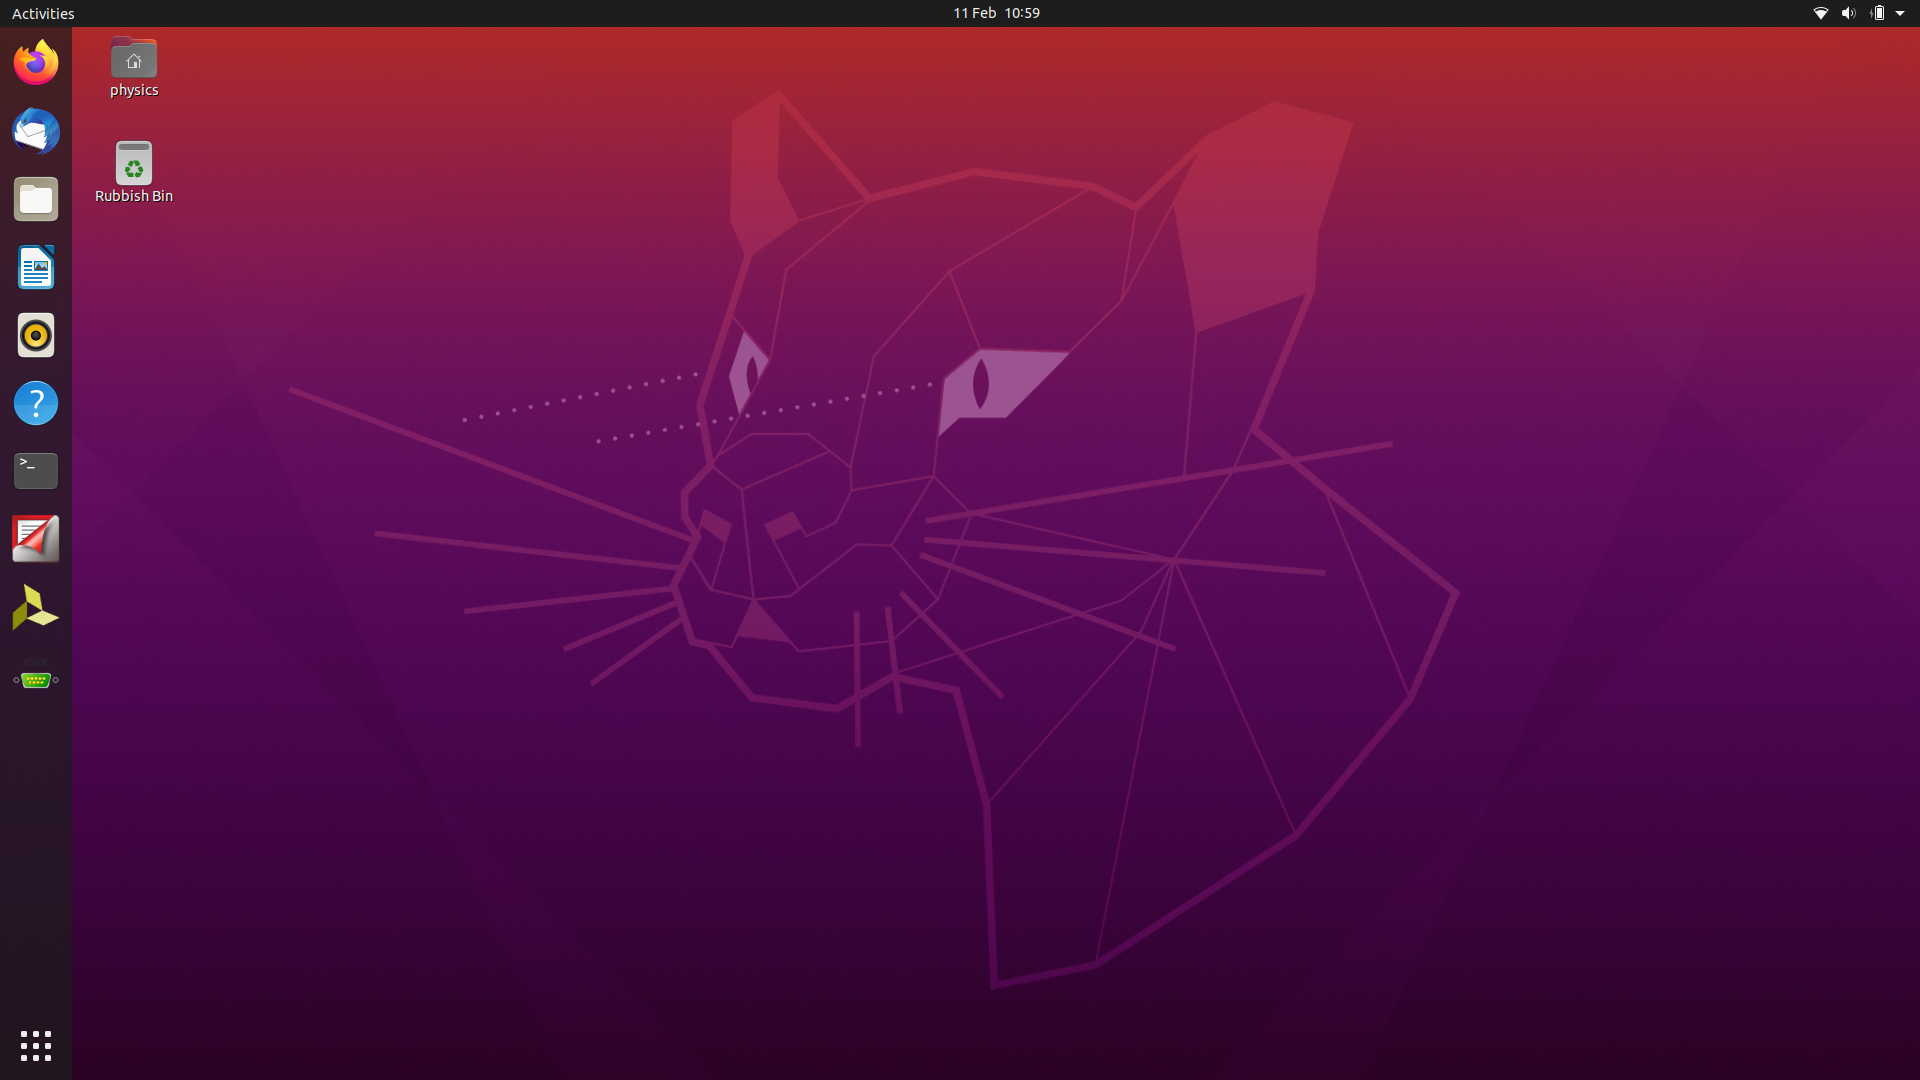
\includegraphics[width=\textwidth]{figures/blank_ubuntu_screen.png}
    \caption{A blank screen upon logging in as physics to Ubuntu}
    \label{fig:emptyscreen}
\end{figure}

You can single-left-click on any of these items to run the corresponding applications. If you run something and want to stop, just as in Windows, use the red 'x' in the top right hand corner of the window. Most windows can be resized by dragging on the corners, minimised by clicking on the underscore also in the top right corner, and expanded to full-screen mode by clicking on the rectangle in the same place. If you minimise a window belonging to one of the sidebar applications, it can be recovered by clicking again on the icon. You can also re-open a minimised icon by clicking on 'Activities' in the top left hand corner. The full set of installed applications can be seen by clicking on `nine dots' icon in the lower left corner. You can drag across the mouse pad to go up and down the full set of icons. Clicking on it again takes you back. If you are alone and want some background music or talk, the 'RythmnBox' application plays podcasts. 

The two icons in the top left of the main window are short-cuts to the Files application running on your home directory and the contents of the rubbish bin

Firefox should need no explanation. The `Files' application is like the Windows file manager, and it allows you to navigate through the hierachy of folders on the Ubuntu machine. If you right click on a file you are given an option to move to the recycle bin, just as in Windows. In fact, Ubuntu is trying to emulate the Windows operating system. The big difference between Linux and Windows is the use of the Terminal application. Windows has the DOS prompt, but DOS is so arcane that few but the brave use it very much. In Linux the Terminal 'shell' is the BASH shell, which has quite a lot of functionality and is quite sophisticated. However, you shouldn't actually need to learn too much UNIX/Linux to do this course. If you are interested, there are lots of tutorials on line in learning the BASH shell in UNIX/Linux. The serial port terminal will be useful later in the course when we are communicating with microprocessor cores on the BASYS3 board. Vivado and Vitis are the two graphical user interfaces that we will use to develop our applications. We will spend most of our time using Vivado and Vitis.

Before you can use Firefox you will need to connect your laptop to a wireless network. The icon to do this is in the top right hand corner of the screen and looks like a segment of fruit. If you click on this icon it will show you a list of available wireless networks - you should check and see that there is one that you can log in to. After logging in, the segment will be partially filled in, indicating the quality of your connection.

You should be able to use Firefox to log on to MUSE and from there with the google mail tool and Blackboard you should be able to use your laptop to take part in the lab projects without need for your own personal devices. The camera built in to the laptop and the built in microphone both work with blackboard and we will need to communicate with each other freely to make a success of the course, within the limits imposed by bandwidth.

To shut the laptop down, the small downwards arrow in the very top right pulls down a menu from which you can select the Power Off/Log Out option, and there you can do all the usual things - turn off, restart, log out, etc. In these things Ubuntu again behaves much like other popular operating systems.

There are also several other equipment items. These are, all told
\begin{enumerate}
    \item Cardboard box and packing material (please preserve in good condition)
    \item Laptop with power supply (two connected cables)
    \item Gel filled protective laptop case
    \item USB to micro-usb adaptor cable
    \item Basys3 FPGA development board
    \item PMODDAC2 two channel digital-to-analog converter (DAC) - this is small!
    \item some cables
    \item a crystal earpiece
\end{enumerate}

Obviously try not to lose anything and tell me if you do, or if anything gets broken. Try NEVER to keep drinks anywhere they can spill on the laptop. Especially on the table directly next to them. Think of them as lab equipment. You wouldn't drink in a lab, so don't keep drinks in the vicinity of this machinery.

One final thing about the laptops. If you want to dump the whole screen to a picture file, then at any time you can just press the PrtScr button which is on your keyboard two keys to the right of the space bar, and a `.png' format bitmap of the entire screen is written to the Pictures subfolder of your home directory. Try this, and then use the Files application to go to this directory, double clicking on the icon to view it. If you just want to print one window, make sure this window is selected, then hold down the Alt key and again press PrtScr (Alt-PrtScr), and a `.png' file just of the highlighted window is put in the same place. This could be useful if something isn't working right and you want to send myself or Mitch graphics that are useful in explaining your problem.

\end{document}